\documentclass{beamer} 
\usetheme{default} 
\usecolortheme{albatross}
\setbeamercovered{transparent}
%\useoutertheme{umbcfootline}  


\usepackage[spanish]{babel}
%\usepackage[latin1]{inputenc}
\usepackage[utf8x]{inputenc}
\usepackage{hyperref}
\usepackage{color}



%\usepackage{multicol}




\title{Excepciones en java}

\author{Manuel J. Molino Milla \and Luis Molina Garzón}

\date{\today} %

\institute{IES Virgen del Carmen \and Departamento de Informática}




%\beamerdefaultoverlayspecification{<+->}

\begin{document}


\begin{frame}
  \titlepage
\end{frame}

\begin{frame}
    \frametitle{Logo}
\begin{figure}

\includegraphics[scale=1]{imagenes/logo.jpeg} 
\caption{Logo Java}
\end{figure}
\end{frame}

%\begin{frame}
 % \frametitle{Contenido}
 %\tableofcontents[pausesections]
%\end{frame}

\begin{frame}[fragile]
\frametitle{Introducción}
\begin{itemize}[<+->]
\item Una excepción en términos de lenguaje de programación es la indicación de un problema que ocurre durante la ejecución de un programa.
\item  El manejo de excepciones permite al usuario crear aplicaciones tolerantes a fallos.
\item Se puede controlar estas excepciones y que pueda seguir ejecutando el programa sin verse afectado por el problema. 
\item  En lenguaje java estas excepciones pueden manejarse con las clases que extienden el paquete \emph{Throwable} de manera directa o indirecta
\end{itemize}
\end{frame}

\begin{frame}[fragile]
\frametitle{¿Cuando pueden ocurrir?}
Una excepción es un objeto que se genera automáticamente cuando se produce un acontecimiento circunstancial que impide el normal funcionamiento del programa:
\begin{itemize}[<+->]
\item División por cero
\item Intentar leer desde un fichero que no existe.
\item Un error en la conexión de Internet.
\item Un error en el acceso a una base de datos.
\item Un error de lectura/escritura en disco
\item Acceder a una posición de una colección inexistente.
\item ....
\end{itemize}
\pause
El objeto generado “excepción” contiene información sobre el acontecimiento ocurrido y transmite esta información al método desde el que se ha generado la excepción.
\end{frame}

\begin{frame}[fragile]
\frametitle{Ejemplo}
\begin{verbatim}
public class Excepcion1{
        public static void main(String[] arg){
                int numerador= 10;
                int denominador = 0;
                int division = numerador/denominador;
                //....
        }
}
\end{verbatim}
\pause 
\textcolor{orange}{Esto produce:}
\pause
\begin{footnotesize}
\begin{verbatim}
Exception in thread "main" java.lang.ArithmeticException: / by zero
	at Excepcion1.main(Excepcion1.java:5)

\end{verbatim}
\end{footnotesize}
\end{frame}

\begin{frame}
\frametitle{Tipos de excepciones}
\begin{figure}
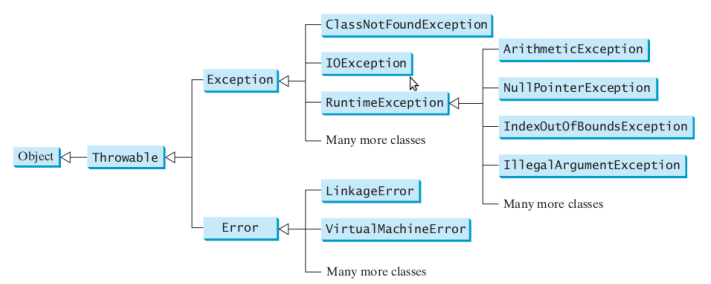
\includegraphics[scale=0.5]{imagenes/excepciones.png}
\end{figure}
\end{frame}

\begin{frame}[fragile]
\frametitle{RunTimeException}
\begin{itemize}[<+->]
\item Aparecen cuando hay un error en el programa.
\item Tal es el caso de dividir por cero o acceder a una posición de una colección que supere el tamaño de la misma.
\item Se conoce también como \emph{Unchecked Exceptions}
\item Este tipo de excepciones no deben tratarse. Debemos evitarlas corrigiendo el programa.
\end{itemize}
\end{frame}

\begin{frame}[fragile]
\frametitle{Ejemplo}
\begin{scriptsize}
\begin{verbatim}
public class Excepcion{
   public static void main(String[] arg){
      int numero = Integer.parseInt(arg[0]);
      //resto de código
   }
}
\end{verbatim}
\pause
\textcolor{orange}{Si no se pasa argumento origina:}
\begin{verbatim}
Exception in thread "main" java.lang.ArrayIndexOutOfBoundsException: 0
	at Excepcion.main(Excepcion.java:3)
\end{verbatim}
\pause
\textcolor{orange}{Mejor:}
\begin{verbatim}
public class Excepcion1{
   public static void main(String[] arg){
      if (arg.length == 0){
          System.out.println("Faltan argumentos");
          System.exit(1);
      }
      int numero = Integer.parseInt(arg[0]);
      //resto de código
   }
}
\end{verbatim}
\pause
\textcolor{orange}{Si falta el argumento produce:}
\begin{verbatim}
Faltan argumentos
\end{verbatim}
\end{scriptsize}
\end{frame}

\begin{frame}[fragile]
\frametitle{Excepciones declarativas}
\begin{itemize}[<+->]
\item Son condiciones excepcionales del flujo del programa pero que no son debido a un error del propio programa. 
\item Si se lanza una excepción \emph{checked} el programa no tiene ningún tipo de error.
\item Y el programa sigue funcionando correctamente.
\item Este tipo de excepciones deben ser tratadas.
\item Si no son tratadas, originan un error de compilación.
\end{itemize}
\end{frame}

\begin{frame}[fragile]
\frametitle{Manejo de excepciones declarativas}
\begin{itemize}[<+->]
\item Se usa el bloque \emph{try-catch-finally}
\item En el bloque \emph{try} se intentará atrapar la excepción para posteriormente tratarla.
\item En el bloque \emph{catch} definimos el conjunto de instrucciones necesarias o de tratamiento del problema capturado con el bloque \emph{try} anterior.
\item El bloque \emph{finally} es opcional, se ejecuta siempre (si hay o no hay excepción). Es buen lugar para cerrar flujos de programa como puede ser un \emph{Scenner} o un descriptor del fichero.
\end{itemize} 
\end{frame}

\begin{frame}[fragile]
\frametitle{Ejemplo}
\begin{verbatim}
Path path = Paths.get("data/subdir");

try {
    Path newDir = Files.createDirectory(path);
} catch(FileAlreadyExistsException e){
    // the directory already exists.
} catch (IOException e) {
    //something else went wrong
    e.printStackTrace();
}
\end{verbatim}
\end{frame}

\begin{frame}[fragile]
\frametitle{Ejemplo}
\begin{verbatim}
try {
  InputStream input = new FileInputStream("c:\\data\\...");
  System.out.println("File opened...");

} catch (IOException e){
  System.err.println("File opening failed:");
  e.printStackTrace();
}
\end{verbatim}
\end{frame}

\begin{frame}[fragile]
\frametitle{Ejemplo}
\begin{verbatim}
URLConnection connection = new URL(url).openConnection();
connection.setDoOutput(true); // Triggers POST.
connection.setRequestProperty("Accept-Charset", charset);
connection.setRequestProperty("Content-Type", 
"application/x-www-form-urlencoded;charset=" + charset);

try (OutputStream output = connection.getOutputStream()) {
    output.write(query.getBytes(charset));
}

InputStream response = connection.getInputStream();
// ...
\end{verbatim}
\end{frame}

\begin{frame}[fragile]
\frametitle{Bloque finally}
\begin{small}
\begin{itemize}[<+->]
\item A veces interesa lanzar un trozo de código independientemente que se lancen o no excepciones dentro de un bloque try.
\item Generalmente son operaciones relacionadas con recuperación de memoria.
\item Para esto se usa la clausula \alert{finally}
\item En Java el recolector de basura se encarga la liberacion de objetos no referenciados, por lo que la liberacion de memoria no es problema.
\item Pero \emph{finally} es muy recomendado para cerrar los flujos de I/O
\end{itemize}
\pause
\begin{verbatim}
try{
    actividades peligrosas A y B
}catch(A a1){
    manejador de la situación de A
}catch(B b1){
    manejador de la situación de B
}finally{
    actividades que se van a realizar
}
\end{verbatim}
\end{small}
\end{frame}

\begin{frame}[fragile]
\frametitle{Ejemplo}
\begin{verbatim}
FileInputStream in = null;
......  
try {
   in = new FileInputStream(...);  // Open stream
   ......
   ......
} catch (IOException ex) {
   ex.printStackTrace();
} finally {  // always close the I/O streams
   try {
      if (in != null) in.close();
   } catch (IOException ex) {
      ex.printStackTrace();
   }
}
\end{verbatim}
\end{frame}


\begin{frame}[fragile]
\frametitle{Ejemplo finally}
\begin{scriptsize}
\begin{verbatim}
class Excepcion extends Exception{}
public class EjemploFinally{
  static int contador = 0;
  public static void main (String[]arg){
    while (true)
      {
        try
        {
          if (contador++ == 0)
            throw new Excepcion ();
            System.out.println ("Sin excepción");
        }
        catch (Excepcion e)
        {
          System.err.println ("Excepción");
        }
        finally
        {
          System.err.println ("Inicio de clausula finally");
          if (contador == 2)
            break;
        }
      }
  }
}
\end{verbatim}
\end{scriptsize}
\end{frame}

\begin{frame}[fragile]
\frametitle{Usando java post 1.7}
No se usa la clausula \emph{finally}, los flujos se cierran solo si se definen al lado del \emph{try}
\begin{verbatim}
try (FileInputStream in = new FileInputStream(...)) {
   ......
   ......
} catch (IOException ex) {
   ex.printStackTrace();
}  //Automatically closes all opened resource in try (...).
\end{verbatim}
\end{frame}


\begin{frame}[fragile]
\frametitle{Relanzar una excepción}
\begin{itemize}[<+->]
\item La gestión de excepciones anteriores se denomina \emph{captura de excepción}
\item Otra alternativa es relanzar la excepción.
\item En caso de querer relanzar la excepción, debemos declarar dicha intención en el final del método que contiene las sentencias que lanzan la excepción.
\item Lo hacemos mediante la claúsula \alert{throws}.
\item Esta indica una o una lista de excepciones.
\item Hay que tener presente que cuando se relanza una excepción estamos forzando a nuestro método a capturarla o relanzarla.
\item Una excepción que sea relanzada una y otra vez hacia arriba terminará llegando al método primigenio.
\item En caso de no ser capturada por éste, producirá la finalización de su hilo de ejecución (thread).
\end{itemize}
\end{frame}

\begin{frame}

\frametitle{Excepciones mas comunes en Java}
\begin{description}[<+->]
\item[AritmeticException] En operaciones aritméticias
\item[ArrayIndexOutOfBoundsException] Fuera del límite de un \emph{array}
\item[ClassCastException] Casting incorrecto
\item[IlegalArgumentException] Argumento no válido en la llamada de un método.
\item[IndexOutOfBoundsException] Índice fuera de una colección.
\item[NegativeArraySizeException] Tamaño menor que cerro en un \emph{array}
\item[NullPointerException] Uso de una referencia nula.
\item[NumberFormatException] Formato de número incorrecto.
\item[StringIndexOutOfBoundException] Índice de un String fuera de su longitud.
\item[IOException] Error de entrada/salida
\item[SQLException] Errores en el manejo de sentencias SQL.
\item[\dots]
\end{description}
\end{frame}

\begin{frame}[fragile]
\frametitle{Creando excepciones propias}
\begin{itemize}[<+->]
\item El programador puede lanzar sus propias excepciones
\item Las expcepciones son objetos, por lo que debemos generar una clase que cree dichos objetos.
\item Dicha clase debe extender de la clase Exception. Debemos usar la sintáxis \emph{extends Exception} para crear las nuevas \emph{excepciones}
\item Tenemos constructores que podemos pasar un mensaje como argumento.
\item Varios métodos, entre otros \emph{printStackTrace()} que se invoca cuando no tratamos la excepción.
\item Lanzamos las excepciones usando \emph{throw}
\item Pero el método que crea la excepción debe indicar en su declaración que puede lanzar dicha excepción, para esto usa el comando \emph{throws}
\end{itemize}
\end{frame}

\begin{frame}[fragile]
\frametitle{Ejemplo}
\begin{scriptsize}

\begin{verbatim}
public class TestTrianguloRectangulo {
   public static void main(String[] ar) throws NoTrianguloRectanguloException {
      TrianguloRectangulo t1 = new TrianguloRectangulo(1, 1, 2);
      TrianguloRectangulo t2 = new TrianguloRectangulo(1, 2, 5);
   }
}

class TrianguloRectangulo{
    private double cateto1;
    private double cateto2;
    private double hipotenusa;
    public TrianguloRectangulo(double cateto1,
           double cateto2, double hipotenusa) throws
    NoTrianguloRectanguloException{
        if (Math.pow(cateto1,2)+Math.pow(cateto2,2)==
            Math.pow(hipotenusa,2)){
            this.cateto1=cateto1;
            this.cateto2=cateto2;
            this.hipotenusa=hipotenusa;
        }
        else
            throw new NoTrianguloRectanguloException();
    }
}
class NoTrianguloRectanguloException extends Exception{}
\end{verbatim}

\end{scriptsize}
\end{frame}
\end{document}